See quadrilateral $ABCD$ in Fig.\ref{fig:2.2.6_quad_1} is generated using the following python code 
\begin{lstlisting}
solutions/6/codes/quadrilateral/quad.py
\end{lstlisting}
\begin{figure}[!ht]
\centering
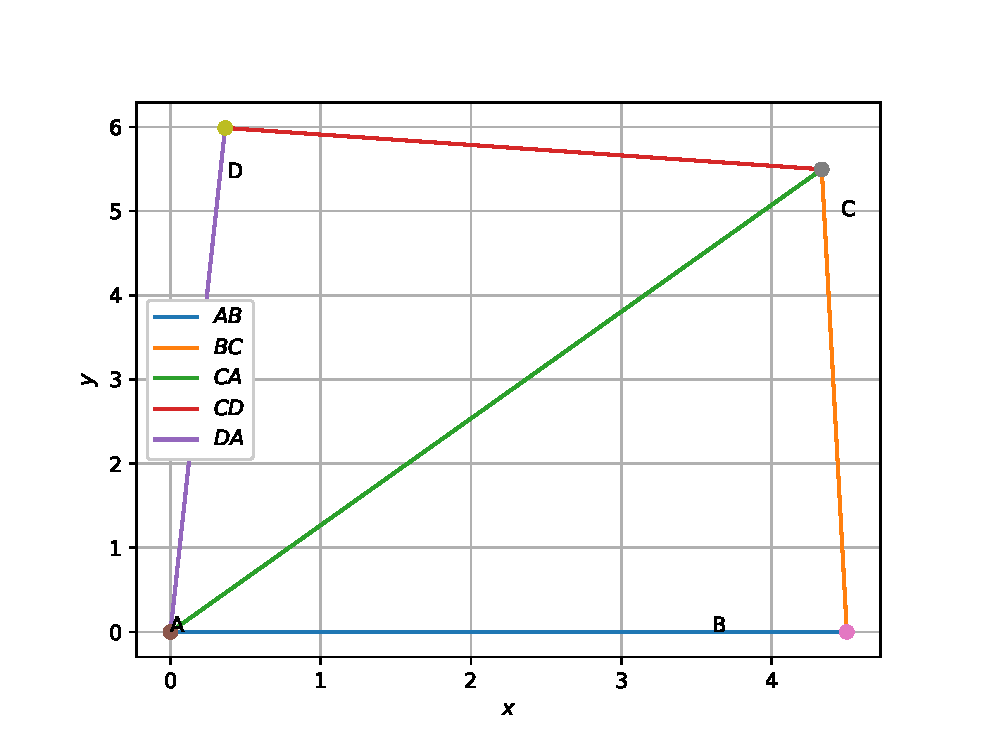
\includegraphics[width=\columnwidth]{./solutions/6/codes/quadrilateral/quad.eps}
\caption{Quadrilateral $ABCD$ using python}
\label{fig:2.2.6_quad_1}
\end{figure} 
%
\begin{align}
ar\brak{ABCD} &= ar\brak{\triangle ABC} + ar\brak{\triangle {ACD}}
\\
&=\frac{1}{2}\norm{(\vec{B}-\vec{A})\times(\vec{C}-\vec{A})}
\\
&\quad +\frac{1}{2}\norm{(\vec{C}-\vec{A})\times(\vec{D}-\vec{A})}
%
\\
&=\frac{1}{2}\norm{\myvec{1\\-7} \times \myvec{7\\-4}} 
\\
&\quad +\frac{1}{2}\norm{\myvec{7\\-4} \times \myvec{6\\1}} 
\\
&= 38
\end{align}
and verified using the following codes
\begin{lstlisting}
solutions/6/codes/tri_area_ABC.py
\end{lstlisting} 
\begin{lstlisting}
solutions/6/codes/tri_area_ACD.py
\end{lstlisting} 

